% Backup slides, after "Thank you!": for questions. Numbered B1, B2, ...
% (preamble: \backuppart), not counted in the talk's total.
\backuppart

\begin{frame}
  \frametitle{Conjugate Hylomorphisms}
  \begin{center}
    {\Large\emph{Every recursion scheme is a conjugate hylomorphism}}
    \vspace{.4cm}

    \begin{sticky}
      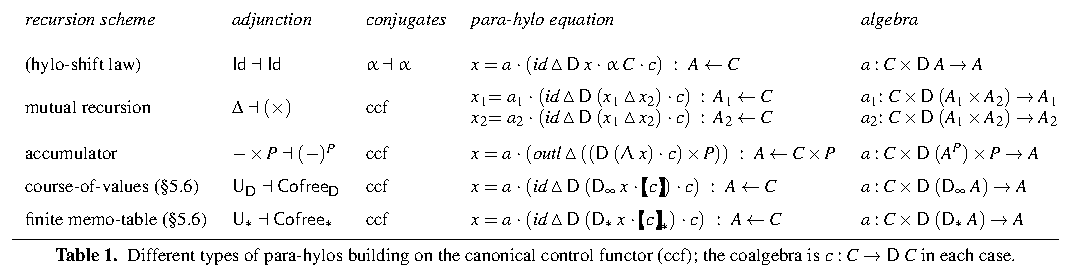
\includegraphics[width = \textwidth, alt = {Table 1 of Hinze, Wu and
        Gibbons: para-hylos built on the canonical control functor, for the
        hylo-shift law, mutual recursion, accumulators, course-of-values
        recursion and finite memo-tables, with their adjunctions,
        conjugates, equations and algebras.}]{types-of-parahylos-crop.pdf}
    \end{sticky}
  \end{center}
  \slideref{R. Hinze, N. Wu, J. Gibbons. \textbf{Conjugate Hylomorphisms, or: The Mother of All Structured Recursion Schemes}. POPL 2015.}
  \speakernote{Accumulators: curry/uncurry \\ Dynamic programming: cofree
      comonad}
\end{frame}

\begin{frame*}
  \frametitle{Proving Hylomorphisms Correct}
  \rocqblock{hylo-ind.v}
  \simplified
  \begin{itemize}
    \item Induction on the termination proof; unroll \code{hylo} once
      (\code{hylo\_unr}).
    \item Proved once for the specification, carried along every
      calculation step.
  \end{itemize}
  \speakernote{QSort.v: sorted and permutation}
\end{frame*}

\begin{frame*}
  \frametitle{Terminal Coalgebras and Finite Trees}
  \rocqblock{gfix.v}
  \simplified
  \begin{itemize}
    \item \code{GFix}: bisimilarity with Paco; anamorphisms into it, with
      their universal property.
    \item A coalgebra is recursive iff its anamorphism only builds finite
      trees.
    \item \code{rana}: straight into the initial algebra, no conversion.
  \end{itemize}
  \speakernote{Terminal class, as Initial \\ rana\_ana: rana and ana
      agree}
\end{frame*}

\begin{frame*}
  \frametitle{CPS Coalgebras in Rocq}
  \rocqblock{cps.v}
  \simplified
  \begin{itemize}
    \item \code{hylo\_cps} takes any \code{CCoalg c}: the CPS law is a
      field. The slides' $\cps{c}$ is \code{cps\_from\_coalg}'s.
    \item \code{RecF\_inv\_eq}: a match on \code{E}, so the recursion stays
      structural on \code{H}.
  \end{itemize}
  \speakernote{HyloCPS.v \\ tsplit\_k : CCoalg tsplit, by cps\_from\_coalg}
\end{frame*}

\begin{frame*}
  \frametitle{Coalgebras Need Not Follow the Data}
  \rocqblock{digits.v}
  \begin{center}
    \begin{tikzpicture}[alt={The digits coalgebra on 13 in base 2: 13
        gives digit 1 and seed 6, 6 gives digit 0 and seed 3, 3 gives
        digit 1 and seed 1, 1 gives digit 1 and seed 0, and 0 stops.},
      node distance = 12mm]
      \node[box] (a) {$13$};
      \node[box, right = of a] (b) {$6$};
      \node[box, right = of b] (c) {$3$};
      \node[box, right = of c] (d) {$1$};
      \node[box, right = of d] (e) {$0$};
      \draw[->] (a) -- node[above, note] {1} (b);
      \draw[->] (b) -- node[above, note] {0} (c);
      \draw[->] (c) -- node[above, note] {1} (d);
      \draw[->] (d) -- node[above, note] {1} (e);
      \node[note, right = 3mm of e] {digits of $13 = 1101_2$};
    \end{tikzpicture}
  \end{center}
  \ocamlblock{fastpow.ml}
  \speakernote{Power: fold over the binary digits \\ Deforested: fast
      exponentiation}
\end{frame*}

\begin{frame*}
  \frametitle{Knapsack: the \texttt{Derive}}
  \rocqblock{knap-derive.v}
  \speakernote{Side goals: the loop's step, its first entry, the lookup
      algebra}
\end{frame*}

\begin{frame}
  \frametitle{What Changed Since the Paper}
  \begin{itemize}
    \item Rocq 9; properness and termination by instance search; an Elpi
      coercion for curried morphisms.
    \item \code{Derive}, \code{arewrite} and \code{finished} for
      calculations; CPS coalgebras for extraction.
    \item \code{Initial} and \code{Terminal} classes; \code{RecF} iff
      \code{well\_founded (child c)}; \code{GFix} with Paco.
    \item Finite containers and monoid algebras; dynamorphisms over
      arrays.
    \item New examples: MSS, fast power, knapsack.
  \end{itemize}
  \speakernote{Library: github.com/dcastrop/rocq-hylomorphisms}
\end{frame}
